\chapter{Implementation of The Data Pipeline}
\section*{Introduction}
\addcontentsline{toc}{section}{Introduction}

This chapter introduces a comprehensive pipeline designed to collect
and process data for our nutrition application. We start by the data
understanding phase, which involves collecting and exploring the data
to identify potential problems. Then, we detail the data preparation
phase, which includes the implementation of an ETL pipeline to clean,
transform, and load the data into a structured format suitable for use by
the recommendation system and the AI assistant. The data is collected
from various European retailers using web scraping techniques that we
will present it with details in a separated section. The collected data is
then cleaned, transformed, and enriched with additional features such as
the Nutri-Score, dietary labels, and other relevant nutritional indicators.
In the final stage, the processed data is embedded and stored in a vector
database to enable efficient semantic search.
\section{Data Understanding}
Following the Business Understanding phase outlined in the first
chapter, we now advance through the remaining CRISP-DM steps.
This section focuses on the Data Understanding phase, which involves
collecting and exploring the data to identify potential problems.

\subsection{Sources}

\par The data used comes mainly from web scraping of a wide variety of
food products in Europe. We scraped data from the websites of major
supermarkets in France, Italy, Germany, and Spain.
The scraped data includes detailed product information and nutritional
values such as calories, carbohydrates, fats, and proteins, as well as
ingredients and allergens.


\subsection{Problems} 
After solving the problem of missing data by building the ML model Nutri-pred-V1, we still face several challenges related to data quality and consistency.
The discarded products are diverse and inconsistent, as they come from
several countries and different distributors.
One major challenge in our project is that product descriptions are
written in different languages, which complicates product matching and
recommendation. As shown in Figure 3.1, the product description is in
Italian, while other products have descriptions in French, German, or
Spanish. As a result, we need to implement a multilingual approach
to handle these variations effectively. The descriptions show various
inconsistencies, while essential information, including NutriScore and
nutritional labels, is absent from the data.
As a result, an ETL pipeline is required to collect, process, and unify all
products into a consistent database structure.
\begin{figure}[H]
    \centering
    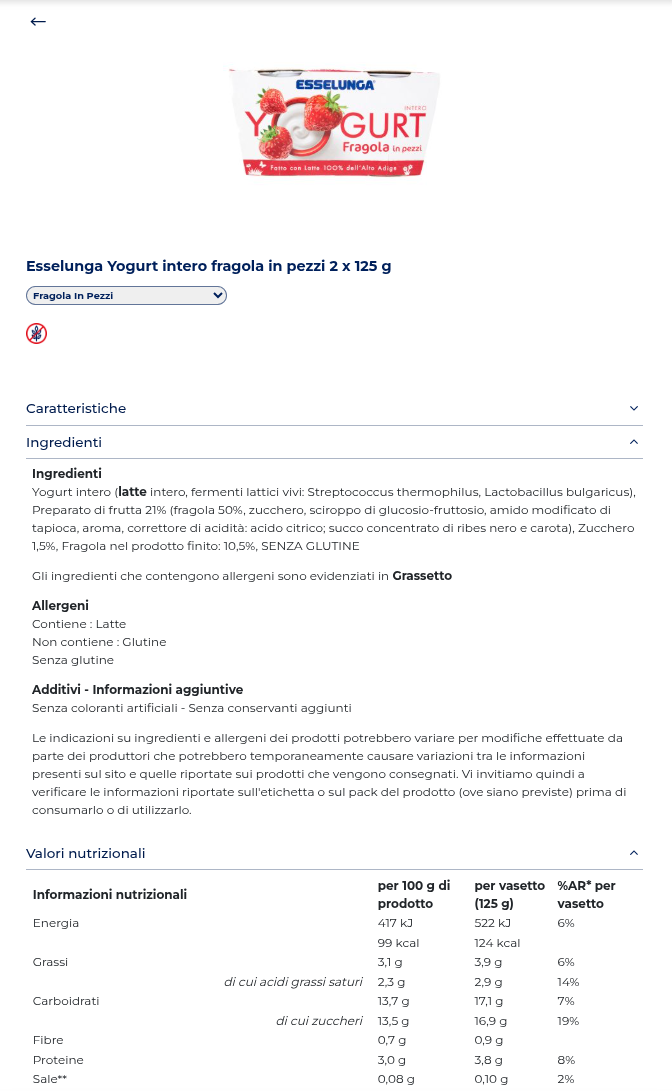
\includegraphics[scale=0.45]{images/product_example.png}
    \caption{An example of a product details page to scrape from the Italian supermarket chain Esselunga} 
    \label{fig:scraped_data}
\end{figure}


\subsection{Data enrichment}
Another challenge is the nutritional evaluation of each product. It is
impractical to manually assess each product by identifying high-sugar
items for individuals with diabetes or detecting products that do not
contain gluten for people with celiac disease. After the web scraping, the
data pipeline must automatically add pertinent health labels and nutrition
indicators like the Nutri-Score in order to solve this problem. This feature
engineering is a crucial step for enabling efficient product filtering and
delivering personalized recommendations. In parallel, data is enriched
with behavioral data from users’ browsing history on the app, including
products viewed, liked, or disliked, as well as user profiles describing their
dietary preferences, allergies, medical conditions or nutritional goals.

\section{Data preparation: ETL pipeline}


The data preparation phase is a crucial step in the CRISP-DM methodology, as it directly impacts the quality and effectiveness of the subsequent
modeling phase. During this phase, we implement an ETL pipeline to
clean, transform, and load the data into a structured format suitable for
use by the recommendation system and the AI assistant. This section
details the technical aspects of the ETL process that was implemented
to collect, process, and integrate products from various European stores,
as well as the tools and methodologies used in this step.

\begin{center}
\begin{figure}[H]
    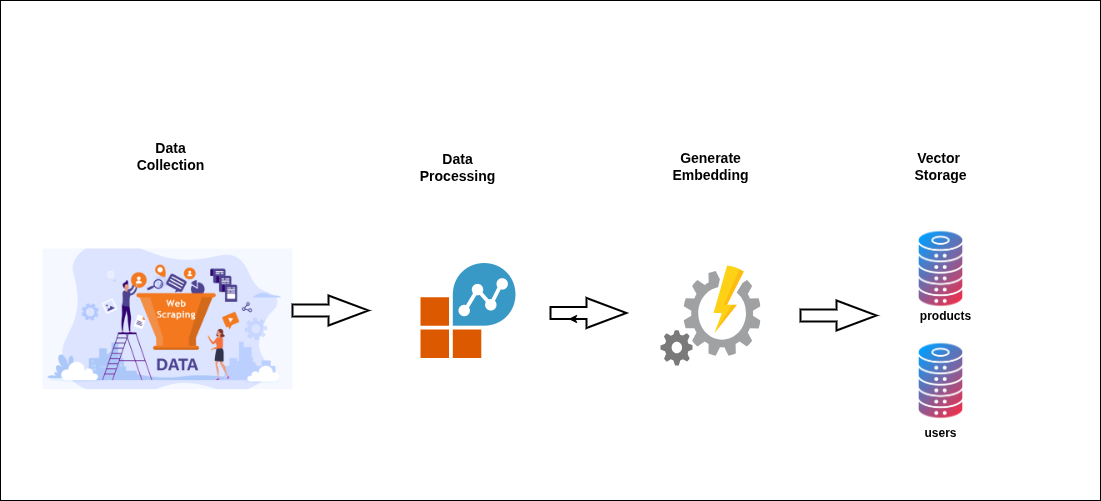
\includegraphics[scale=0.39]{images/workflow__data.png}
    \caption{End-to-end data workflow: from web scraping to vector embedding}
    \label{fig:data_workflow}
\end{figure}
\end{center}

\subsection{Extract}

\par The starting point in the ETL processing workflow is the data extraction phase. It includes gathering nutritional information, prices, and
descriptions from a range retailer websites using web scraping.
\par Despite the variety of websites available in Europe for scraping, there
are many challenges. The retailers websites have different structures and
categories of products. Selecting the appropriate CSS selectors or HTML
tags for each relevant piece of information is therefore a critical step.
These challenges will be examined in greater detail in the subsequent
section on web scraping.
\par The scraped data, as illustrated in Figure \ref{fig:scraped_data}, is initially stored in a raw format as JSON files. This raw data serves as the foundation for subsequent processing and transformation steps.
\begin{center}
\begin{figure}[H]
\centering
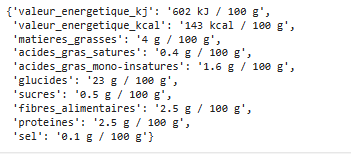
\includegraphics[scale=0.66]{images/nutrition.png}
\caption{Example of a nutrition column before processing} 
\label{fig:Nutrition_column}
\end{figure}
\end{center}

\subsection{Transform}
After that, The gathered data is cleaned, enriched, and standardized
during the transformation phase to guarantee accuracy and compatibility with VitamiNurse’s requirements.
The scraper provided us with comprehensive product information, including many irrelevant columns. We will extract only the relevant product columns to simplify and focus our
analysis.

\subsubsection{Data Cleaning}
We performed a thorough cleaning. To do this, we removed columns
containing products with duplicate EAN codes to eliminate redundancies
and ensure data quality. We also decided to remove columns with
empty nutritional values. Nutritional information was originally located
under the main column "evolutions". We extracted this information and
reorganized it into a separate "nutrition" column, using a dictionary
format.


\subsubsection{Normalization and transformation}

We had to process the "nutrition" column of our database, since it included detailed nutritional information such as energy, fat, carbohydrates,
protein, and salt for each product. For example, here is an entry from
the "nutrition" column.

\begin{center}
\begin{figure}[H]
    \centering
    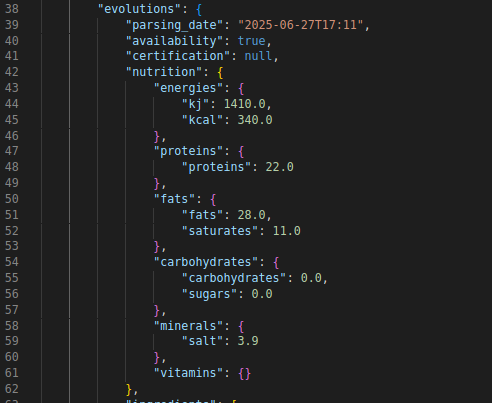
\includegraphics[scale=0.45]{images/transform_nutrition.png}
    \caption{Example of a nutrition column after Normalization and Transformation} 
    \label{fig:Normalization_nutrition}
\end{figure}
\end{center}

\par It was necessary to normalize these data to ensure that they were on
the same scale. Normalization allows feature values to be rescaled so
that they fall within a common range. This is particularly important
for recommendation algorithms, which are sensitive to differences in
magnitude between features.

\par The nutritional values were originally expressed in different units, such as
grams (g), milligrams (mg), and kilocalories (kcal). To ensure consistency,
we converted all nutritional values to a standard unit per 100 grams
of product. As we can see in Figure 3.4, nutrition values are now
standardized per 100g after being scraped from the Conad website. This
standardization allows for direct comparison between products in the
next chapter during the recommendation process.

\subsubsection{Feature engineering}
\par Feature engineering involves creating new features or modifying existing
ones to improve the performance of product evaluation and recommendation algorithms.

\par As a next step, we constructed a reference dictionary containing specific
keyword lists, such as ingredients that contain gluten, non-vegetarian
components, pork-derived ingredients, and substances to avoid during
pregnancy. These lists are used to generate customized binary features
for each product, enabling the model to make more personalized and
context-sensitive recommendations.

\begin{center}
\begin{figure}[H]
    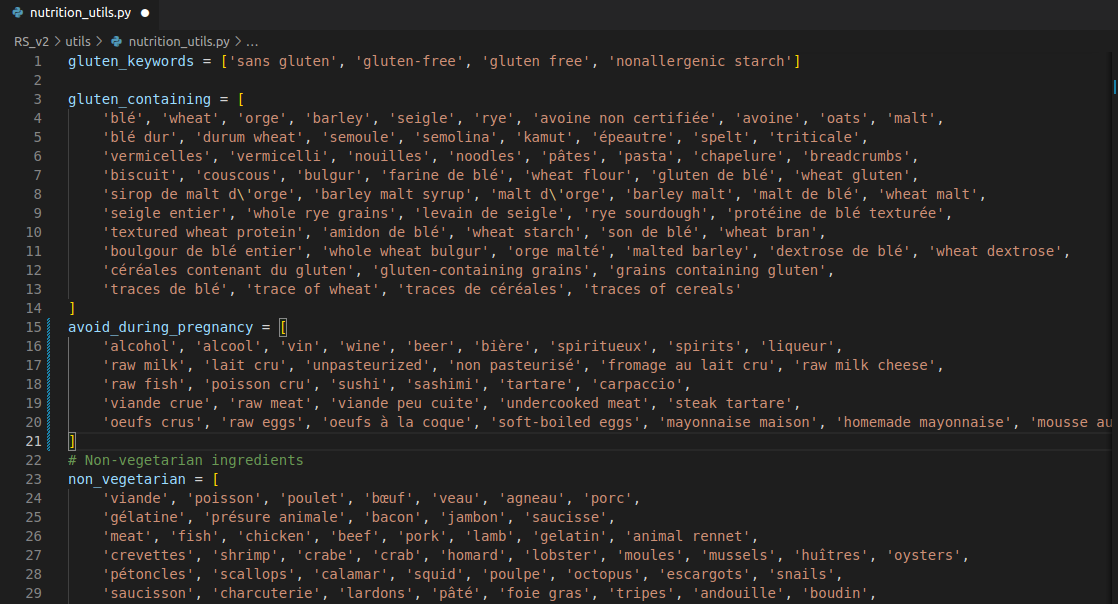
\includegraphics[scale=0.45]{images/nutrition_utils.png}
    \caption{Keywords Dictionary for Automated Nutrition Labelling} 
    \label{fig:nutrition_utils_file}
\end{figure}
\end{center}

After that we combine all the product titles, ingredients, and categories
and check if it matches any specific nutrition keywords from our reference. If a match is found, we assign the corresponding label to the product (e.g., "gluten-free," "ibs-friendly," "vegetarian," "vegan," "halal," "kosher," "pregnancy-safe," etc.). This automated labeling process enhances the product metadata, making it easier to filter and recommend products in real-time based on individual dietary needs and preferences.

\par In addition to checking for keywords, we also analyze the nutrition values of each product to assign dietary labels such as "low sugar," "low fat," or "high protein" based on established nutritional guidelines. This dual approach of keyword matching and nutritional analysis ensures that each product is accurately labeled according to its health attributes, enhancing the recommendation system's ability to cater to individual dietary needs.

 \subsubsection{Adding Nutri-Score}
The last step in the feature engineering process is the computation and assignment of the
Nutri-Score to each product here. The Nutri-Score is a nutrition label that was first implemented in France
in 2017. It features a five-color scale accompanied by letters from A (most
nutritious) to E (least nutritious). It is designed to provide consumers
with clear and immediate information about the nutritional quality of
food products [12]. As discussed in the Nutri-Score FAQ document [13]
developed by the French Public Health Agency, the system is adapted to
align with dietary guidelines throughout Europe. In the data pipeline,
we implemented a function that automatically calculates the Nutri-Score
for each product based on its nutritional values. This function follows
the official Nutri-Score algorithm, which considers both negative and
positive nutritional factors to determine the final score.

%\begin{center}
%\begin{figure}[H]
%    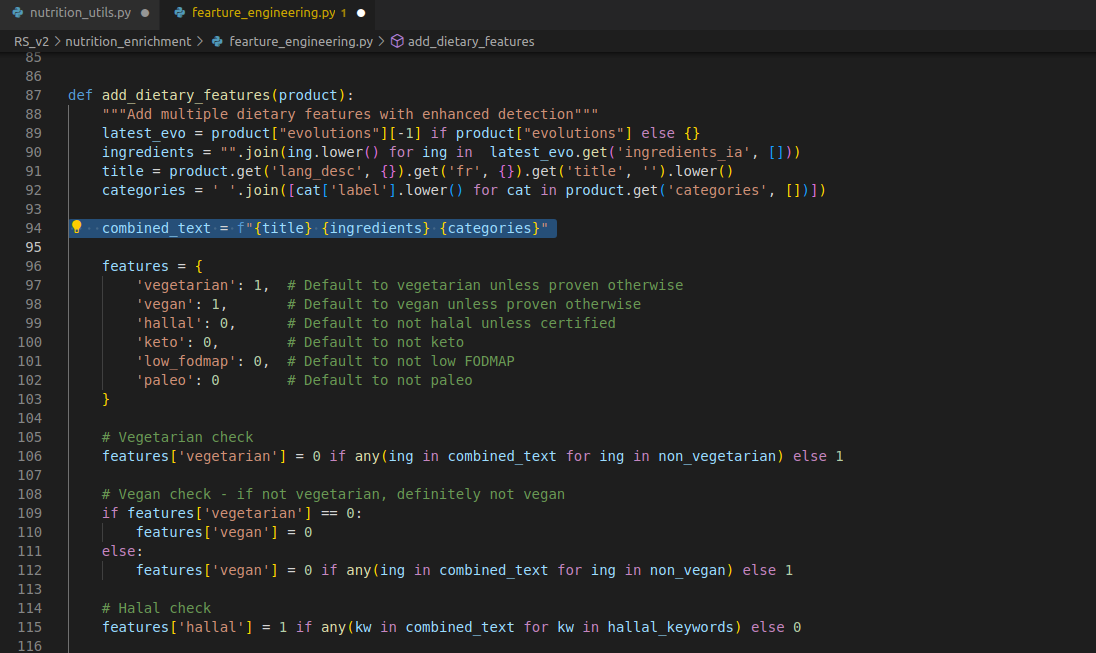
\includegraphics[scale=0.35]{images/feature_engineering.png}
%    \caption{feature engineering} 
%    \label{fig: feature engenieering}
%\end{figure}
%\end{center}


\begin{center}
\begin{figure}[H]
    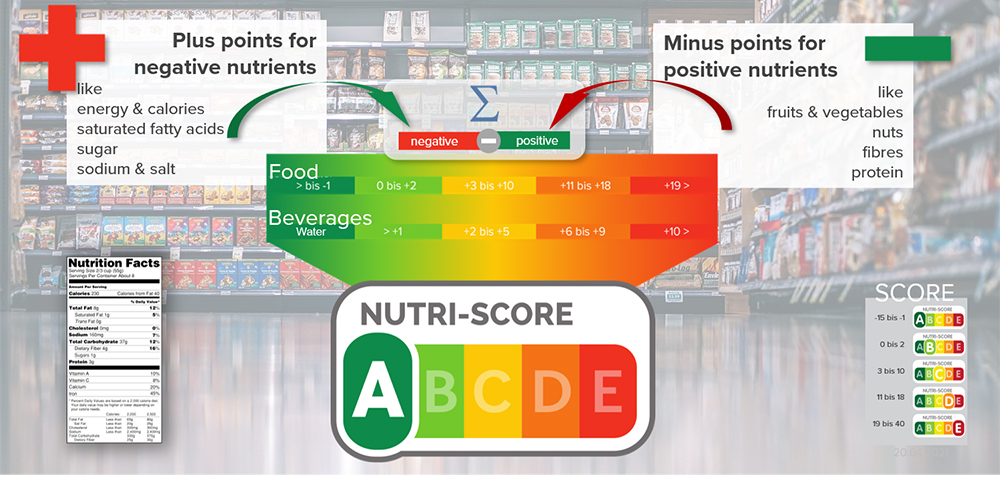
\includegraphics[scale=0.90]{images/nutriscore.jpg}
    \caption{Nutri-Score calculation logic} 
    \label{fig: add_nutriscore}
\end{figure}
\end{center}

\subsection{Load: Data Storage}
After cleaning and transforming the data using an ETL pipeline, the final
phase involves loading the processed information into two complementary
databases to optimize both storage and retrieval.

\subsection{Primary Storage in MongoDB}
As illustrated in Figure\ref{fig:load_data_mongo}, the scraped data are initially stored in MongoDB that serves as the primary database for centralized storage and management. 
This choice guarantees data persistence and reliability, thereby minimizing the risk of data loss while enabling flexible access for subsequent processing stages.


\begin{center}
\begin{figure}[H]
    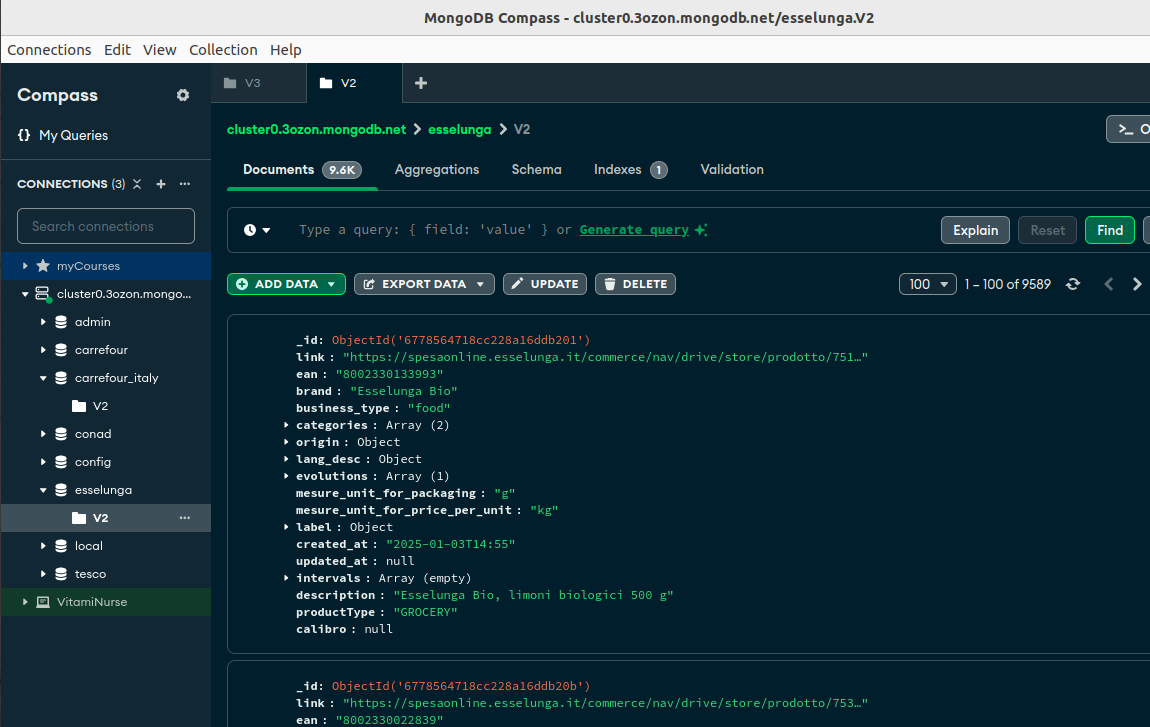
\includegraphics[scale=0.35]{images/load_data.png}
    \caption{Load products for each market in MongoDB} 
    \label{fig:load_data_mongo}
\end{figure}
\end{center}

\subsection{Optimized Vector Store in ChromaDB}
Following data transformation, a refined copy of the users and products
collections is generated, containing only essential attributes such as
the product name, category, and nutritional information. In order to
optimize retrieval and analysis, this database is then embedded and
stored in ChromaDB. This vector database enables similarity search,
allowing the application to easily access and utilize it for further analysis
or recommendation.


\subsection{Dual-database architecture}
 
This dual-database architecture ensures that the system can efficiently
handle structured queries while also enabling advanced recommendation
and conversational features powered by semantic search.

\par The following tools were employed to facilitate data management, em-
bedding generation, and semantic retrieval:

\begin{itemize}[label=\textbf{-}]
    \item \textbf{MongoDB Atlas}: A cloud-hosted NoSQL database service for the efficient storage and management of structured data, offering scalability and ease of deployment in distributed environments.
    \item \textbf{PyMongo}: A robust Python library that enables seamless programmatic interaction with MongoDB instances, supporting operations such as data insertion, querying, and updates.
    \item \textbf{MongoDB Compass}: An intuitive graphical user interface tool for exploring MongoDB collections and visualizing data.
    \item \textbf{ChromaDB}: An open-source vector database optimized for high-dimensional embeddings and enabling efficient similarity searches, particularly suited for semantic querying tasks.
    \item \textbf{SentenceTransformers}: A Python-based library that uses transformer models to generate dense vector representations (embeddings) from textual input.
\end{itemize}


\section{Web scraping}
\par In this section, we detail the web scraping process and tools used to
collect product data from various European retailers. Web scraping is a
technique for extracting information from websites by simulating human
browsing behavior. It is particularly useful for gathering large amounts
of data that are not readily available through APIs or other structured
formats.

\subsection{Web Scraping Process}
\par The web scraping process took place in several successive stages to ensure
efficient information extraction:
\par The first step is the page access. Using Selenium, we automated access
to the various product pages by simulating clicks and navigation between
departments, categories, and subcategories.
\par Then we pass to the information extraction. Once the page loaded, specific information (product name, description, price, images, and storage
instructions) was extracted by analyzing the HTML structure. Particular care was taken to retrieve relevant data, filtering out unnecessary
elements.
The final step is error handling. During scraping, error handling mechanisms were implemented to manage potential page blocks, access restrictions, or changes to the page structure. The main challenge we
encountered is anti-bot management. And we can overcome this problem
by using solutions like random delays, proxy rotation, and user agent
switching.





\subsection{used tools in web scraping}
We have to relied on a complementary set of tools tailored to the diversity
of data sources and formats encountered.

\begin{itemize}[label=\textbf{-}]
    \item \textbf{Selenium:} was used to automate interactions with dynamic web pages, cookie banners or  AJAX scenarios where data loaded via AJAX is not immediately available in the DOM.
    \item \textbf{BeautifulSoup:}  enabled fast and efficient extraction of information from static HTML content.
    \item \textbf{cURL and Requests :} To interact with REST APIs, cURL and Python’s Requests library allowed for simple HTTP requests, sometimes requiring authentication or specific parameters. 
\end{itemize}



\section*{Conclusion}
In conclusion, we can provide a robust foundation for ingesting and processing data from multiple platforms by building a robust data pipeline.
This pipeline ensures that the data is clean, standardized, and enriched
with relevant features, making it suitable for powering the recommendation system and AI assistant. Furthermore, to optimize semantic search
and enable real-time personalized recommendations, we implemented a vector database for efficient data storage and retrieval. To ensure data
completeness and support accurate recommendations, a machine learning model is also trained to predict missing values. 
The next chapters will focus on the recommendation system and the AI assistant, detailing how they leverage this well-prepared data to deliver personalized nutrition advice and product suggestions to users.